%=============================================================================
\section{Design}
\label{sec:design}

%-----------------------------------------------------------------------------
\subsection{Approach}

	zkInterface is a procedural, purely functional interface for zero-knowledge systems that enables cross-language interoperability. The current version, even if limiting, creates an interface based on R1CS formatting and offers the ability to abstractly craft a constraint system building from different gadgets, possibly written in different frameworks, by defining how data should be written and read.
	It is independent of any particular proving systems.

	The same interface can be used in two use-cases:
	\begin{itemize}
		\item To connect the construction and execution of a zero-knowledge program
			to a proving system. See Figure \ref{program_proving}.

		\item To decompose a zero-knowledge program into multiple gadgets that can be engineered separately. See Figure \ref{program_components}.
	\end{itemize}
	
\begin{figure}[!h]
	\centering
	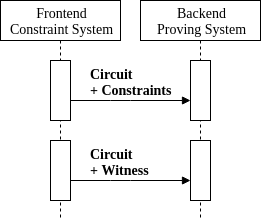
\includegraphics[width=0.5\linewidth]{graphics/program_proving.png}
	\caption{The interaction between a zero-knowledge program and a proving system.}
	\label{program_proving}
\end{figure}

\begin{figure}[!h]
	\centering
	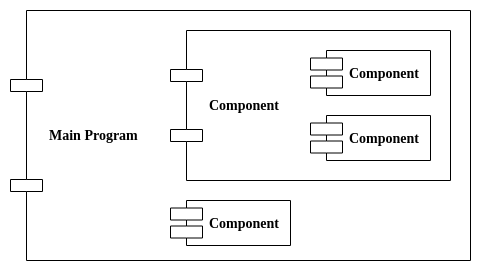
\includegraphics[width=0.7\linewidth]{graphics/program_components.png}
	\caption{A zero-knowledge program built from multiple gadgets.}
	\label{program_components}
\end{figure}


\parhead{Interface}

	The interaction between caller and gadgets is based on exchanging messages.
	Messages are purely read-only data, which grants a great flexibility to
	implementations of gadgets and applications.

\parhead{Interoperability}

	Different parts of an application may be written in different programming languages, and interoperate through messages.
	These parts may be linked and executed in a single process, calling functions,
	and exchanging messages through buffers of shared memory.
	They may also run as separate processes, writing and reading messages in files, or through pipes or sockets.
	Some implementation strategies are discussed in section~\ref{sec:implementation}.

\parhead{Messages Definition \label{message_definition}}

	The set of messages is defined in Listing \ref{gadget.fbs}, 
	using the FlatBuffers interface definition language.
	All messages and fields are defined in this schema.

	The FlatBuffers system includes an interface definition language
	which implies a precise data layout at the byte level.
	Code to write and read messages can be generated for all common programming languages.
	Examples are provided for C++ and for Rust.

	Multiple paths for evolution and extensions of the standard are possible,
	thanks to the flexibility and backward-compatibility features of the encoding.
	The encoding is designed to require little to no data transformation, making it possible
	to implement the standard with minimal overhead in very large applications.

	Messages must be prefixed by the size of the message not including the prefix,
	as a 4-bytes little-endian unsigned integer.
	This makes it possible to concatenate and distinguish messages
	in streams of bytes or in files.

	The specification of FlatBuffers can be found at
	\href{https://google.github.io/flatbuffers/}{https://google.github.io/flatbuffers/}.


\parhead{Instance and Witness Reductions}

	Instance reduction is the process of constructing a constraint system.
	Witness reduction is the process of assigning values to all variables
	in the system before generating a proof about concrete input values.

	When using a proving system with pre-processing, instance reduction
	is performed once ahead of time and used in a trusted setup.
	In proving systems without pre-processing, instance reduction is used in proof verification.
	The standard supports both execution flows.


%-----------------------------------------------------------------------------
\subsection{Architecture}

\begin{figure}[!h]
	\centering
	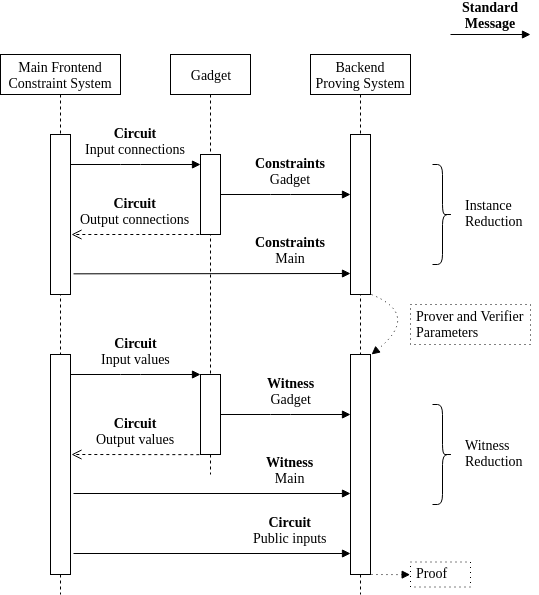
\includegraphics[width=\linewidth]{graphics/call_flow.png}
	\caption{The flow of messages between libraries using the interface.}
	\label{flow}
\end{figure}

\parhead{Messages Flow}

	The flow of messages is illustrated in Figure \ref{flow}.

	The caller calls the gadget code with a single \textsf{GadgetCall} message.
	The gadget exits with a single GadgetReturn message.
	This is a control flow analoguous to a function call in common programming languages.

	The caller also provides a way for the gadget to send
	R1CSConstraints and AssignedVariables messages.
	This is an output channel distinct from the return messages.

	The caller can request an instance reduction, or a witness reduction, or both at once.
	This is controlled by the fields generate\_r1cs and generate\_assignment of GadgetCall messages.

	During instance reduction,
	a gadget may add any number of constraints to the constraint system
	by sending one or more R1CSConstraints messages.
	The caller and other gadgets may do so as well.

	During witness reduction,
	a gadget may assign values to variables
	by sending one or more AssignedVariables messages.

	\subparagraph{Note}
	The design of constraints and assignments channels
	allows a gadget to call subgadgets itself.
	Messages from all (sub-)gadgets can simply be sent separately
	without the need to aggregate them into a single message.
	
	Moreover, an implementation can decouple the proving system
	from the logic of building constraints and assignments,
	by arranging for the constraints and assignments messages
	to be processed by the proving system, independently from the control logic.

\parhead{Variables}
	The constraint system reasons about variables, which are assigned a numerical identifier that are unique within a constraint system. The variable numbers are incrementally allocated in a global namespace. Messages that contain constraints or assignments refer to variables by this numeric ID. It is up to gadgets that create the constrain system to keep track of the semantics (and if desired, helpful symbolic names) of the variables that they deal with, and to allocate new variables for their internal use. The messages defined by the framework include a simple protocol for conveying the state of of the variable allocator (i.e., the first free variable number), and the identity of variables that tie a gadget to other gadgets.

	\subparagraph{Note}
	This design allows implementations to aggregate and handle messages in a generic way,
	without any	reference to the gadgets or mechanisms that generated them.

\parhead{Local Variables Allocation}
	A gadget may allocate a number of local variables to use
	in the internal implementation of the function that it computes.
	They are analoguous to stack variables in common programming languages.

	The following protocol is used to allocate variable IDs that are
	unique within a whole constraint system.
	\begin{itemize}
		\item The caller must provide a numerical ID greater than all IDs that have already been allocated, called the Free-Before ID.
		\item The gadget may use the Free-Before ID and consecutive IDs as its local variables IDs.
		\item The gadget must return the next consecutive ID that it did not use, called the Free-After ID.
		\item The caller must treat IDs lesser than the Free-After ID as allocated by the gadget,
			and must not use them.
	\end{itemize}

	During instance reduction, the gadget can refer to
	its local variables in the R1CSConstraints messages that it generates.
	The caller and other parts of the program must not refer to these local variables.

	During witness reduction, the gadget must assign values to its local variables
	by sending AssignedVariables messages.

\parhead{Incoming/Outgoing Variables}

	The concept of incoming, outgoing variables arises when a program is decomposed into gadgets.
	These variables serve as the functional interface between a gadget and its caller.
	They are analoguous to arguments and return values of functions in common programming languages.
	A variable is not inherently incoming, outgoing, nor local;
	rather, this is a convention in the context of a gadget call.

	The caller provides the IDs of variables to be used as incoming and outgoing variables by the gadget.
	There may be no outgoing variables if the gadget implements a pure assertion.

	During instance reduction, both the caller and the gadget can refer to
	these variables in the R1CSConstraints messages that they generate.
	Other parts of the program may also refer to these same variables in their own contexts.

	During witness reduction, the caller must pass incoming values to the gadget in the GadgetCall message.
	The gadget must return outgoing values to the caller in the GadgetReturn message.

	The caller is responsible for the assignment of values to both incoming and outgoing variables.
	How this is achieved depends on the caller and proving system,
	and on whether some variables are treated as public inputs of the instance.
